\subsection{Thermochimie du lithium}
\label{subsubsection:thermochimie_du_lithium}

\setcounter{equation}{0}
\setcounter{Q}{0}

Le lithium (solide) décompose l'eau avec dégagement de dihydrogène ; la solution obtenue devient basique.

\Q \label{Q:04-01} Donner les demi-équations rédox associées à chacun des couples (le pH sera supposé valoir par la suite 14). En déduire l'équation de réaction.
\solution{Du fait de l'alcalinistion du milieu et de la solubilité de \ce{LiOH}, on est amené à considérer les couples \ce{Li^+ (aq) / Li (s)} et \ce{H2O(l) / H2 (g)}.
\begin{center}
\begin{minipage}{0.4\textwidth}
\begin{align*}
\ce{Li (s) &= Li^+ (aq) + e^-} \\
\ce{H2O (l) + e^- &= \frac{1}{2} H2 (g) + HO^- (aq) } \\
\hline
\ce{Li (s) + H2O (l) &= \frac{1}{2} H2 (g) + Li^+ (aq) + HO^- (aq)}
\end{align*}
\end{minipage}
\end{center}
Au vu des données, \ce{Li^+ (aq)} et \ce{HO^- (aq)} seront considérés ensemble (comme une paire d'ions intime) :
\begin{align*}
\ce{Li (s) + H2O (l) = \frac{1}{2} H2 (g) + (Li^+ , HO^-) (aq)}
\end{align*}
}

\Q Rappeler la relation entre la force électromotrice $e$ et l'enthalpie libre de réaction $\Delta_r G$ à température ambiante et pression standard.
\solution{
Le travail électrique est lié à l'enthalpie libre de réaction par : 
\begin{align*}
\Delta_r G = - F e
\end{align*}
puisqu'un électron est mis en jeu dans l'équilibre de la Q. \ref{Q:04-01}.
En condition standard à température ambiante, on peut écrire : 
\begin{align*}
\Delta_r G^\circ = - F e^\circ
\end{align*}
}
%L’énergie de la réaction à température et pression constantes correspond à l’enthalpie libre de réaction

\Q Calculer la force électromotrice en condition standard.
\solution{La f.e.m. est donnée par : 
\begin{align*}
e^\circ &\stackrel{AN}{=} E^\circ_\oplus - E^\circ_\ominus \\
&= - E^\circ (\ce{Li^+ (aq) / Li (s)})
\end{align*}
}

\Q \label{Q:04-05} En vous appuyant sur un cycle thermodynamique, calculer l'enthalpie libre de réaction puis l'entropie libre de réaction. Rappeler le nom de la loi sur laquelle vous vous êtes appuyez.
\solution{Cycle thermodynamique de Hess : 
\begin{center}
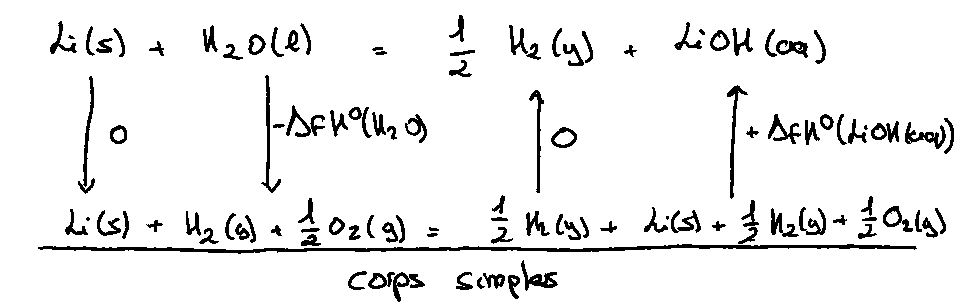
\includegraphics[width=0.8\textwidth]{Ex04/Corr02}
\end{center}
En utilisant la loi de Hess, on a : 
\begin{align*}
\Delta_r H^\circ &= \frac{1}{2} \Delta_f H^\circ ( \ce{H2 (g) } ) + \Delta_f H^\circ (\ce{ LiOH (aq)}) - \Delta_f H^\circ ( \ce{Li (s)} ) - \Delta_f H^\circ ( \ce{H2O (l)} ) \\ 
&= \Delta_f H^\circ (\ce{ LiOH (aq)}) - \Delta_f H^\circ ( \ce{H2O (l)} ) \\
&= -223 ~ \si{\kilo\joule\per\mole} 
\end{align*}
On peut déduire l'entropie de réaction standard de la combinaison linéaire des entropies molaires : 
\begin{align*}
\Delta_r S^\circ &= S^\circ_m ( \ce{LiOH(aq)} ) + \frac{1}{2} S^\circ_m ( \ce{\ce{H2(g)}} ) - S^\circ_m ( \ce{Li(s)} ) - S^\circ_m ( \ce{H2O (l)} ) \\ 
 &= -30.8 ~ \si{\joule\per\mole\per\kelvin}
\end{align*}
}

\Q En déduire l'enthalpie libre standard de réaction à \SI{298}{\kelvin}
\solution{D'après la définition de $G \stackrel{def}{=} H - TS$, on peut en déduire que : 
\begin{align*}
\Delta_r G^\circ = \Delta_r H^\circ - T \Delta_r S^\circ
\end{align*}
\textbf{AN :} $\Delta_r G^\circ = -214 ~ \si{\kilo\joule\per\mole}$
}

\Q \label{Q:04-06} Exprimer la constante de réaction en fonction des activités et, à l'aide de la Q. \ref{Q:04-05}, en déduire la valeur de la constante de réaction à \SI{298}{\kelvin}. Commenter.

\solution{\`{A} l'équilibre chimique, on peut utiliser la loi d'action des masses :
\begin{align*}
Q_{r,eq} = K_r^\circ (T) \implies  \frac{ a^{1/2} ( \ce{H2}) a ( \ce{HO^-} ) a (\ce{Li^+})}{a (\ce{H2O}) a(\ce{Li}) } = K_r^\circ (T)
\end{align*}
En l'absence de travail électrique (les deux couples sont dans le même compartiment) :
\begin{align*}
\Delta_r G \stackrel{eq}{=} 0 &\implies \Delta_r G^\circ (T) + RT \ln Q_{r,eq} = 0 \\
& \implies K_r^\circ (T) = \exp \left( - \frac{\Delta_r G^\circ (T) }{RT} \right)
\end{align*}
\textbf{AN :} $K_r^\circ (298 ~ \si{\kelvin}) = 3.15 \cdot 10^{37}$
Le lithium métallique réagira spontanément (=réaction exergonique) avec l'eau.
}

\Q \'{E}crire le potentiel d'équilibre de chacun des couples et en déduire le potentiel standard du couple \ce{Li^+ (aq) / Li (s)} à \SI{298}{\kelvin}. Commenter la valeur obtenue.
\solution{\`{A} \SI{298}{\kelvin} 
\begin{align*}
E (\ce{Li^+ (aq) / Li (s)}) &= E^\circ (\ce{Li^+ (aq) / Li (s)}) + \alpha \log \left ( \frac{ a ( \ce{Li^+} ) }{ a ( \ce{Li} )} \right) \\
E (\ce{H^+ (aq) / H2 (g)}) &= E^\circ (\ce{H^+ (aq) / H2 (g)}) + \alpha \log \left ( \frac{ a (\ce{H^+})}{a^{1/2} ( \ce{H2})} \right) \\
&= E^\circ (\ce{H^+ (aq) / H2 (g)}) + \alpha \log K_e +\alpha \log \left ( \frac{ a (\ce{H2O})}{a^{1/2} ( \ce{H2}) a(\ce{HO^-})} \right)
\end{align*}
en utilisant la loi des masses sur l'autoprotolyse de l'eau : 
\begin{align*}
K_e = \frac{a ( \ce{H^+ } ) a( \ce{HO^-} )}{a ( \ce{H2O} )}
\end{align*}
\`{A} l'équilibre chimique, en l'absence de travail (les deux couples sont dans le même compartiment) :
\begin{align*}
\Delta_r G \stackrel{eq}{=} 0 &\implies E (\ce{Li^+ (aq) / Li (s)}) \stackrel{eq}{=} E (\ce{H^+ (aq) / H2 (g)}) \\
&\implies E^\circ (\ce{Li^+ (aq) / Li (s)}) = E^\circ (\ce{H^+ (aq) / H2 (g)}) + \alpha \log K_e - \alpha \log K_r^\circ
\end{align*}
\textbf{AN :} $E^\circ (\ce{Li^+ (aq) / Li (s)}) = -3.1 \si{\volt\per{ESH}}$ avec 2 C.S.
Au regard des autres espèces chimiques rédox, rencontrées en chimie des solutions, le lithium est un élément très réducteur.
}

Le potentiel de Nernst (1889) du couple \ce{Li^+ (aq) / Li (s)} correspond à la force électromotrice (f.e.m.) aux bornes de la pile \og factice \fg{} suivante :
\begin{align*}
\ce{Pt (s)} | \ce{H2(g)} | \ce{H^+ (aq)} || \ce{Li+ (aq)} | \ce{Li (s)} | \ce{Pt (s)} 
\end{align*}
avec la demi-pile de gauche constituée de l'électrode standard à hydrogène \ce{H^+ (aq)}/\ce{H2 (g)} (ESH). 

Selon la convention de Latimer, $E^\circ (\ce{H^+(aq)} / \ce{H2(g)} ) = 0$. Le couple \ce{H^+(aq)} / \ce{H2(g)} est dit \og  silencieux \fg{}.

\Q Justifier le sens du terme \og factice \fg{}.
\solution{
Le terme factice sous-entend que cette pile n'existe pas en réalité pour deux raisons : 
\begin{itemize}
\item toutes les conditions d'une ESH, rappelées dans le polycopié du cours, ne peuvent être réalisées ; 
\item la demi-pile lithium ne peut être réalisée sans destruction complète de l'électrode par l'eau.
\end{itemize}
}

\Q En supposant que cette pile puisse être réalisée, schématiser-la et orienter-la.
\solution{Le potentiel du lithium étant plus réducteur que celui de l'eau, on peut proposer l'orientation suivante : 
\begin{center}
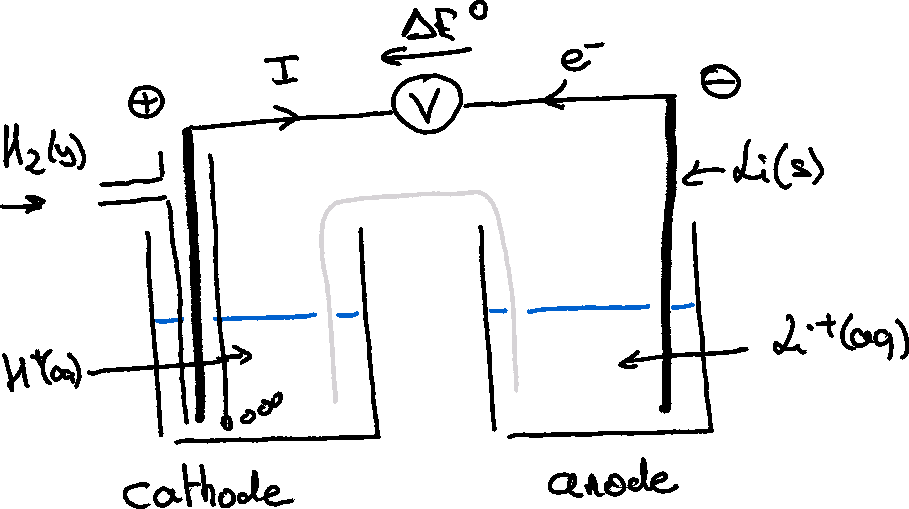
\includegraphics[width=0.5\textwidth]{Ex04/Corr01}
\end{center}
avec $P_{\ce{H2}} = P^\circ$ et $[\ce{Li^+}] = [\ce{H^+}] = c^\circ$. La f.e.m. est donnée par :
\begin{align*}
\Delta E^\circ = E_\oplus^\circ - E_\ominus^\circ = 3.1 ~ \si{\volt}
\end{align*}
}

\Q Conclure quant à l'intérêt d'utiliser du lithium métallique comme anode dans les piles au lithium (technologie Li-métal).
\solution{
En l'absence d'eau et de contact avec l'atmosphère, le lithium présente un caractère très réducteur vis-à-vis de la plupart des espèces chimiques connues. On peut donc espérer, en le plaçant au sein d'une batterie, convertir l'énergie chimique en énergie électrique (plutôt qu'en chaleur, comme lorsqu'il réagit avec l'eau).
}

\subsection*{Données à \SI{298}{\kelvin}}
\begin{itemize}
\item Enthalpie standard de formation et entropie molaire standard :
\begin{center}
\begin{tabular}{ccccc}
\toprule
& \ce{H2O(l)} & \ce{Li(s)} & \ce{(Li^+ ,  HO^-)(aq)} & \ce{H2(g)} \\
\midrule
$\Delta_f H^\circ$ [\si{\kilo\joule\per\mole}] & -285 & 0 & -508 & 0 \\
$S_m^\circ$ [\si{\joule\per\mole\per\kelvin}] & 69.9 & 29.1 & 2.7 & 131 \\
\bottomrule
\end{tabular}
\end{center}
\item \ce{LiOH} est soluble dans l'eau à température et pression ambiante.
\item $\alpha = \frac{RT}{F} \ln 10 = 0.059 ~ \si{\volt}$
\end{itemize}

